% This file was created by matlab2tikz.
%
%The latest updates can be retrieved from
%  http://www.mathworks.com/matlabcentral/fileexchange/22022-matlab2tikz-matlab2tikz
%where you can also make suggestions and rate matlab2tikz.
%
\definecolor{mycolor1}{rgb}{0.00000,0.44700,0.74100}%
\definecolor{mycolor2}{rgb}{0.85000,0.32500,0.09800}%
\definecolor{mycolor3}{rgb}{0.92900,0.69400,0.12500}%
\definecolor{mycolor4}{rgb}{0.49400,0.18400,0.55600}%
\definecolor{mycolor5}{rgb}{0.46600,0.67400,0.18800}%
%
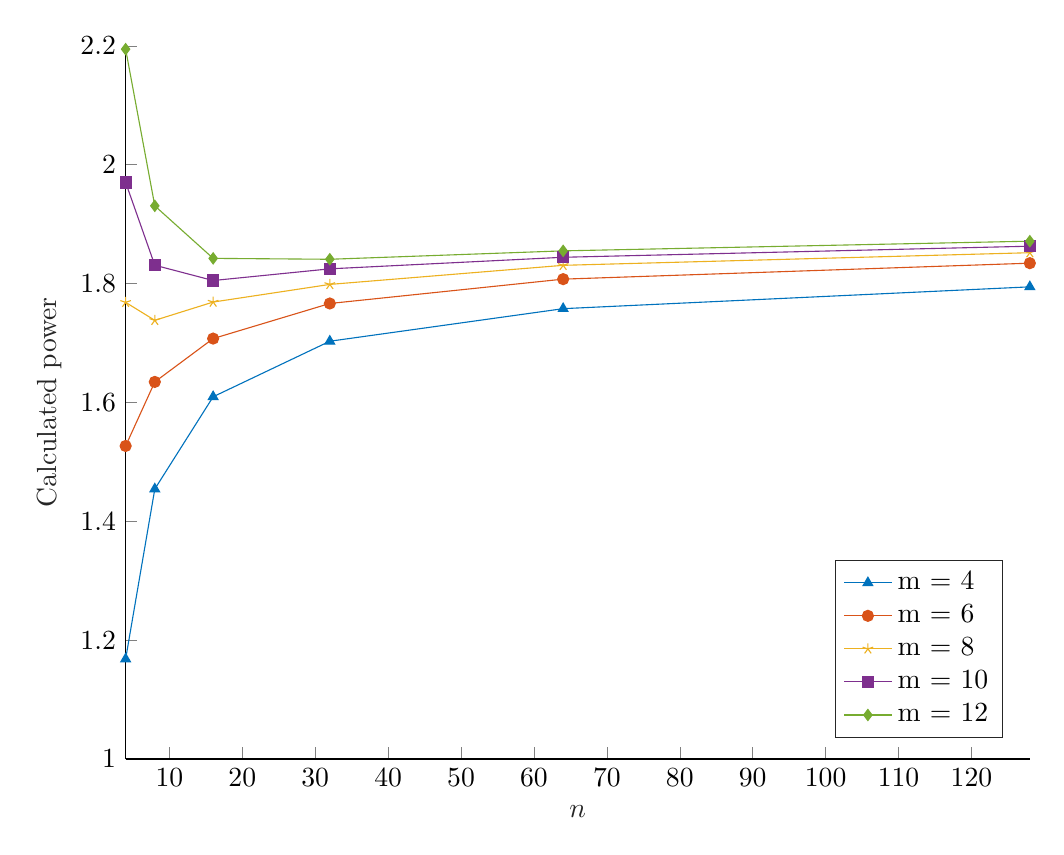
\begin{tikzpicture}

\begin{axis}[%
width=4.521in,
height=3.566in,
at={(0.758in,0.481in)},
scale only axis,
xmin=4,
xmax=128,
xlabel style={font=\color{white!15!black}},
xlabel={$n$},
ymin=1,
ymax=2.2,
ylabel style={font=\color{white!15!black}},
ylabel={Calculated power},
axis background/.style={fill=white},
title style={font=\bfseries},
%title={Power of n in the time complexity. On n 	imes m grid. (free slots = 0.60)},
axis x line*=bottom,
axis y line*=left,
legend style={at={(0.97,0.03)}, anchor=south east, legend cell align=left, align=left, draw=white!15!black}
]
\addplot [color=mycolor1, mark=triangle*]
  table[row sep=crcr]{%
4	1.16825595775638\\
8	1.45427818307774\\
16	1.60949002208362\\
32	1.70292797918649\\
64	1.75772571875204\\
128	1.79443653148065\\
};
\addlegendentry{m = 4}

\addplot [color=mycolor2, mark=*]
  table[row sep=crcr]{%
4	1.52669470977232\\
8	1.63449393712087\\
16	1.70740912197037\\
32	1.7664291390553\\
64	1.80740263069388\\
128	1.83426069032436\\
};
\addlegendentry{m = 6}

\addplot [color=mycolor3, mark=star]
  table[row sep=crcr]{%
4	1.76838703374193\\
8	1.73809860144295\\
16	1.76884464964081\\
32	1.79853102987737\\
64	1.83065246343264\\
128	1.85187284803352\\
};
\addlegendentry{m = 8}

\addplot [color=mycolor4, mark=square*]
  table[row sep=crcr]{%
4	1.97013036703456\\
8	1.83083565662713\\
16	1.80506313875018\\
32	1.82473737732626\\
64	1.8441916760735\\
128	1.86282241932279\\
};
\addlegendentry{m = 10}

\addplot [color=mycolor5, mark=diamond*]
  table[row sep=crcr]{%
4	2.19438407632209\\
8	1.93071231624011\\
16	1.84236138613216\\
32	1.84083283959075\\
64	1.85498009685298\\
128	1.87126670279901\\
};
\addlegendentry{m = 12}

\end{axis}
\end{tikzpicture}%